\chapter{Specifikacija programske potpore}
		
	\section{Funkcionalni zahtjevi}			
			
			\noindent \textbf{Dionici:}
			
			\begin{packed_enum}
				
				\item Administrator
				\item Voditelj natjecanja				
				\item Natjecatelj
				\item Razvojni tim
				
			\end{packed_enum}
			
			\noindent \textbf{Aktori i njihovi funkcionalni zahtjevi:}
			
			
			\begin{packed_enum}
				\item  \underbar{Administrator (inicijator) može:}
				
				\begin{packed_enum}
					
					\item pregledati korisnike
					\item pregledati natjecanja
					\item pregledati zadatke
					\item mijenjati prava korisnicima
					\item promjena podataka korisnika
					\item uređivanje zadataka
					\item uređivanje natjecanja
					
				\end{packed_enum}
			
				\item  \underbar{Neregistrirani korisnik (inicijator) može:}
				
				\begin{packed_enum}
					
					\item se registrirati u sustav
					
				\end{packed_enum}

				\item  \underbar{Voditelj natjecanja (inicijator) može:}
				
				\begin{packed_enum}
					
					\item kreirati nove zadatke
					\item kreirati nova natjecanja
					\item pregledati svoje osobne podatke
					
				\end{packed_enum}

				\item  \underbar{Natjecatelj (inicijator) može:}
				
				\begin{packed_enum}
					
					\item pristupiti natjecanjima
					\item pregledati svoje osobne podatke
					\item pregledati zadatke
					\item predati rješenje zadatka
					\item izrada virtualnog natjecanja
					\item pregled rješenja zadataka
					
				\end{packed_enum}

				\item  \underbar{Baza podataka (sudionik):}
				
				\begin{packed_enum}
					
					\item pohranjuje sve podatke o korisnicima
					\item pohranjuje sve podatke o natjecanjima i zadacima
					
				\end{packed_enum}
			\end{packed_enum}

			\eject 
			
			
				
			\subsection{Obrasci uporabe}
				
				
				\subsubsection{Opis obrazaca uporabe}
					

					\noindent \underbar{\textbf{UC1 - Pregled početne stranice}}
					\begin{packed_item}
	
						\item \textbf{Glavni sudionik: }Korisnik
						\item  \textbf{Cilj:} Odlučiti se za opciju registracije ili prijave
						\item  \textbf{Sudionici:} Baza podataka
						\item  \textbf{Preduvjet:} -
						\item  \textbf{Opis osnovnog tijeka:}
						
						\item[] \begin{packed_enum}
	
							\item Prikazuje se početna stranica
							\item Odabir prijave ili registracije
							\item Prosljeđivanje na odabranu opciju
							
						\end{packed_enum}
					\end{packed_item}
					
					\noindent \underbar{\textbf{UC2 - Registracija}}
					\begin{packed_item}
						
						\item \textbf{Glavni sudionik: }Neregistrirani korisnik
						\item  \textbf{Cilj:} Odlučiti se za opciju registracije kao voditelj ili natjecatelj 
						\item  \textbf{Sudionici:} Baza podataka
						\item  \textbf{Preduvjet:} -
						\item  \textbf{Opis osnovnog tijeka:}
						
						\item[] \begin{packed_enum}
							
							\item Prikazuje se stranica za registraciju
							\item Neregistrirani korisnik ispunjava zadane podatke
							\item Odabire opciju registracije za voditelja ili natjecatelja
							\item Potvrđivanje registracije putem email-a
							\item Dodatna potvrda administratora za novog voditelja
							
						\end{packed_enum}
						
						\item  \textbf{Opis mogućih odstupanja:}
						
						\item[] \begin{packed_item}
							
							\item[2.a] Odabir već zauzetog korisničkog imena i/ili e-maila, unos korisničkog podatka u nedozvoljenom formatu ili pružanje neispravnoga e-maila
							\item[] \begin{packed_enum}
								
								\item Sustav odbija odobravanje registracije
								\item Korisnik mijenja podatke u ispravan unos ili odustaje od registracije 
								
							\end{packed_enum}
						\end{packed_item}
					\end{packed_item}
					
					\eject
					
					\noindent \underbar{\textbf{UC3 - Prijava u sustav}}
					\begin{packed_item}
						
						\item \textbf{Glavni sudionik: }Registrirani korisnik
						\item  \textbf{Cilj:} Prijava u sustav i pristup korisničkom sučelju 
						\item  \textbf{Sudionici:} Baza podataka
						\item  \textbf{Preduvjet:} Registracija
						\item  \textbf{Opis osnovnog tijeka:}
						
						\item[] \begin{packed_enum}
							
							\item Prikazuje se stranica za prijavu
							\item Unos emaila i lozinke
							\item Pristup korisničkoj stranici
							
						\end{packed_enum}
						
						\item  \textbf{Opis mogućih odstupanja:}
						
						\item[] \begin{packed_item}
							
							\item[2.a] Neispravan unos emaila ili lozinke
							\item[] \begin{packed_enum}
								
								\item Sustav odbija pristup te nudi ponovni pokušaj za prijavu
								
							\end{packed_enum}
						\end{packed_item}
					\end{packed_item}
					
					\noindent \underbar{\textbf{UC4 - Pregled osobnih podataka}}
					\begin{packed_item}
						
						\item \textbf{Glavni sudionik: }Natjecatelj, voditelj
						\item  \textbf{Cilj:} Pregledati osobne podatke
						\item  \textbf{Sudionici:} Baza podataka
						\item  \textbf{Preduvjet:} Korisnik je prijavljen u sustav
						\item  \textbf{Opis osnovnog tijeka:}
						
						\item[] \begin{packed_enum}
							
							\item Pritisak korisnika na svoj profil
							\item Prikaz osobnih podataka
							
						\end{packed_enum}
					\end{packed_item}
					
					\noindent \underbar{\textbf{UC5 - Pregled zadataka}}
					\begin{packed_item}
						
						\item \textbf{Glavni sudionik: }Natjecatelj, voditelj
						\item  \textbf{Cilj:} Pregledati zadatke na stranici
						\item  \textbf{Sudionici:} Baza podataka
						\item  \textbf{Preduvjet:} Korisnik je prijavljen u sustav
						\item  \textbf{Opis osnovnog tijeka:}
						
						\item[] \begin{packed_enum}
							
							\item Korisnik pritiskom na dostupne zadatke dobiva pristup
							\item Korisnik može pregledavati već objavljene zadatke
							
						\end{packed_enum}
					\end{packed_item}
					
					\eject
					
					\noindent \underbar{\textbf{UC6 - Pregled kalendara}}
					\begin{packed_item}
						
						\item \textbf{Glavni sudionik: }Natjecatelj, voditelj
						\item  \textbf{Cilj:} Pregledati kalendar 
						\item  \textbf{Sudionici:} Baza podataka
						\item  \textbf{Preduvjet:} Korisnik je prijavljen u sustav
						\item  \textbf{Opis osnovnog tijeka:}
						
						\item[] \begin{packed_enum}
							
							\item Korisnik na svojoj stranici ima pristup kalendaru
							\item Korisnik unutar kalendara može pregledati datume s dostupnim natjecanjima
							
						\end{packed_enum}
					\end{packed_item}
					
					\noindent \underbar{\textbf{UC7 - Pregled profila drugih korisnika}}
					\begin{packed_item}
						
						\item \textbf{Glavni sudionik: }Natjecatelj, voditelj
						\item  \textbf{Cilj:} Pregledati profile drugih korisnika
						\item  \textbf{Sudionici:} Baza podataka
						\item  \textbf{Preduvjet:} Korisnik je prijavljen u sustav
						\item  \textbf{Opis osnovnog tijeka:}
						
						\item[] \begin{packed_enum}
							
							\item Korisnik na svojoj stranici odabire profil koji želi vidjeti
							\item Ako je pritisnuti profil natjecatelj prikazuje se statistika o zadatcima i osvojeni pehari
							\item Ako je pritisnuti profil voditelj prikazuje se popis učitanih zadataka i kalendar s popisom natjecanja
							
						\end{packed_enum}
					\end{packed_item}
					
					\noindent \underbar{\textbf{UC8 - Sudjelovanje u natjecanju}}
					\begin{packed_item}
						
						\item \textbf{Glavni sudionik: }Natjecatelj
						\item  \textbf{Cilj:} Prikazati natjecatelju zadatke za odabrano natjecanje
						\item  \textbf{Sudionici:} Baza podataka
						\item  \textbf{Preduvjet:} Korisnik je prijavljen u sustav i postoji natjecanje u kojem može sudjelovati
						\item  \textbf{Opis osnovnog tijeka:}
						
						\item[] \begin{packed_enum}
							
							\item Natjecatelj sudjeluje u natjecanju
							\item Završetkom natjecanja zadaci postaju dostupni svim korisnicima za vježbanje
							\item Objava rang liste i dodjeljivanje pehara za prva tri mjesta
							
						\end{packed_enum}
						
						\item  \textbf{Opis mogućih odstupanja:}
						
						\item[] \begin{packed_item}
							
							\item[2.a] Pokušaj sudjelovanja u natjecanju korisnika koji nije natjecatelj
							\item[] \begin{packed_enum}
								
								\item Sustav odbija sudjelovanje voditelja u natjecanju 
								
							\end{packed_enum}
						\end{packed_item}
					\end{packed_item}
					
					
					\noindent \underbar{\textbf{UC9 - Kreiranje natjecanja}}
					\begin{packed_item}
						
						\item \textbf{Glavni sudionik: }Voditelj
						\item  \textbf{Cilj:} Voditelj stvara natjecanje  
						\item  \textbf{Sudionici:} Baza podataka
						\item  \textbf{Preduvjet:} Korisnik je prijavljen u sustav i odobren kao voditelj
						\item  \textbf{Opis osnovnog tijeka:}
						
						\item[] \begin{packed_enum}
							
							\item Voditelj ispunjava formu za izradu natjecanja
							\item Voditelj odabire željene zadatke za natjecanje
							\item Natjecanje se kreira i sprema u bazu podataka
							
						\end{packed_enum}
						
						\item  \textbf{Opis mogućih odstupanja:}
						
						\item[] \begin{packed_item}
							
							\item[2.a] Pokušaj kreiranja natjecanja korisnika koji nije voditelj
							\item[] \begin{packed_enum}
								
								\item Sustav odbija kreiranje natjecanja i šalje poruku da korisnik nema ovlasti za taj postupak 
								
							\end{packed_enum}
						\end{packed_item}
					\end{packed_item}
					
					\noindent \underbar{\textbf{UC10 - Kreiranje zadatka}}
					\begin{packed_item}
						
						\item \textbf{Glavni sudionik: }Voditelj
						\item  \textbf{Cilj:} Voditelj stvara zadatak 
						\item  \textbf{Sudionici:} Baza podataka
						\item  \textbf{Preduvjet:} Korisnik je prijavljen u sustav i odobren kao voditelj
						\item  \textbf{Opis osnovnog tijeka:}
						
						\item[] \begin{packed_enum}
							
							\item Voditelj ispunjava formu za izradu zadatka
							\item Voditelj unosi naziv, opis zadatka, testne primjere, broj bodova koji nosi zadatak te ih prosljeđuje sustavu
							\item Voditelj odabire opciju privatnog zadatka, on će postati javan tek nakon završetka natjecanja
							\item Sustav pohranjuje zadatak u bazu podataka
							
						\end{packed_enum}
						
						\item  \textbf{Opis mogućih odstupanja:}
						
						\item[] \begin{packed_item}
							
							\item[2.a] Pokušaj kreiranja zadatka korisnika koji nije voditelj
							\item[] \begin{packed_enum}
								
								\item Sustav odbija kreiranje zadatka i šalje poruku da korisnik nema ovlasti za taj postupak 
								
							\end{packed_enum}
						\end{packed_item}
					\end{packed_item}
					
					\eject
					
					
					\noindent \underbar{\textbf{UC11 - Predaja rješenja zadatka}}
					\begin{packed_item}
						
						\item \textbf{Glavni sudionik: }Natjecatelj
						\item  \textbf{Cilj:} Natjecatelj predaje svoje rješenje zadatka 
						\item  \textbf{Sudionici:} Baza podataka
						\item  \textbf{Preduvjet:} Korisnik je prijavljen u sustav 
						\item  \textbf{Opis osnovnog tijeka:}
						
						\item[] \begin{packed_enum}
							
							\item Natjecatelj šalje zahtjev za evaulaciju rješenja
							\item Evaulator prosljeđuje compileru zahtjev
							\item Compiler pokreće testne primjere nad programom
							\item Evaulator računa broj bodova nakon dobivenih rezultata od compilera
							\item Sustav ažurira broj bodova za natjecatelja i pohranjuje ih u bazu
							
						\end{packed_enum}
						
						\item  \textbf{Opis mogućih odstupanja:}
						
						\item[] \begin{packed_item}
							
							\item[2.a] Natjecatelj ne predaje rješenje zadatka
							\item[] \begin{packed_enum}
								
								\item Natjecatelj ne predaje rješenje zadatka te se ne pokreće proces ocjenjivanja već dodjeljuje 0 
								
							\end{packed_enum}
						\end{packed_item}
					\end{packed_item}
				
					
					\noindent \underbar{\textbf{UC12 - Pregled učitanih rješenja}}
					\begin{packed_item}
						
						\item \textbf{Glavni sudionik: }Natjecatelj
						\item  \textbf{Cilj:} Natjecatelj pregledava rješenja drugih natjecatelja 
						\item  \textbf{Sudionici:} Baza podataka
						\item  \textbf{Preduvjet:} Korisnik je prijavljen u sustav i natjecanje u kojem je sudjelovao je završilo
						\item  \textbf{Opis osnovnog tijeka:}
						
						\item[] \begin{packed_enum}
							
							\item Natjecatelj odabire zadatak unutar natjecanja
							\item Prikazuje mu se popis svih natjecatelja koji su učitali neko rješenje
							\item Rješenja su prikazana sortirano 
							\item Ako je natjecatelj potpuno točno riješio zadatak pojavljuje se opcija za preuzimanje rješenja
							
						\end{packed_enum}
					\end{packed_item}
					
					\eject
					
					\noindent \underbar{\textbf{UC13 - Vježbanje zadataka}}
					\begin{packed_item}
						
						\item \textbf{Glavni sudionik: }Natjecatelj
						\item  \textbf{Cilj:} Natjecatelj ima mogućnost vježbanja već objavljenih zadataka 
						\item  \textbf{Sudionici:} Baza podataka
						\item  \textbf{Preduvjet:} Korisnik je prijavljen u sustav
						\item  \textbf{Opis osnovnog tijeka:}
						
						\item[] \begin{packed_enum}
							
							\item Natjecatelj odabire popis objavljenih zadataka
							\item Natjecatelj pritiskom otvara zadatak koji želi vježbati
							\item Nakon rješavanja zadatka učitava programski kod u aplikaciju
							\item Natjecatelju se dodjeljuju bodovi proporcionalno broju točno riješenih primjera 
							
						\end{packed_enum}
						
						\item  \textbf{Opis mogućih odstupanja:}
						
						\item[] \begin{packed_item}
							
							\item[2.a] Natjecatelj ne predaje rješenje zadatka
							\item[] \begin{packed_enum}
								
								\item Natjecatelj ne predaje rješenje zadatka te se ne pokreće proces ocjenjivanja već dodjeljuje 0 
								
							\end{packed_enum}
						\end{packed_item}
					\end{packed_item}
					
					\noindent \underbar{\textbf{UC14 - Izrada virtualnog natjecanja od prošlih natjecanja}}
					\begin{packed_item}
						
						\item \textbf{Glavni sudionik: }Natjecatelj
						\item  \textbf{Cilj:} Natjecatelj ima mogućnost vježbanja na već objavljenim natjecanjima
						\item  \textbf{Sudionici:} Baza podataka
						\item  \textbf{Preduvjet:} Korisnik je prijavljen u sustav
						\item  \textbf{Opis osnovnog tijeka:}
						
						\item[] \begin{packed_enum}
							
							\item Natjecatelj otvara popis prošlih natjecanja
							\item Natjecatelj odabire neko natjecanje
							\item Natjecanje je aktivno samo za njega
							\item Nakon završetka natjecatelja se rangira po službenim rješenjima 
							
						\end{packed_enum}
					\end{packed_item}
					
					\eject
					
					\noindent \underbar{\textbf{UC15 - Izrada virtualnog natjecanja od nasumičnih zadataka}}
					\begin{packed_item}
						
						\item \textbf{Glavni sudionik: }Natjecatelj
						\item  \textbf{Cilj:} Natjecatelj ima mogućnost vježbanja natjecanja uz pomoć objavljenih zadataka simuliranih u natjecanje
						\item  \textbf{Sudionici:} Baza podataka
						\item  \textbf{Preduvjet:} Korisnik je prijavljen u sustav
						\item  \textbf{Opis osnovnog tijeka:}
						
						\item[] \begin{packed_enum}
							
							\item Natjecatelj odabire opciju natjecanja napravljenog od nasumičnih objavljenih zadataka
							\item Zadatci se spremaju u natjecanje ravnomjerno po količini bodova
							\item Natjecanje je aktivno samo za njega
							\item Završetkom natjecanja ima pristup rješenjima zadataka
							
						\end{packed_enum}
					\end{packed_item}
					
					\noindent \underbar{\textbf{UC16 - Pregled korisnika}}
					\begin{packed_item}
						
						\item \textbf{Glavni sudionik: }Administrator
						\item  \textbf{Cilj:} Administrator ima mogućnost pregleda svih korisnika
						\item  \textbf{Sudionici:} Baza podataka
						\item  \textbf{Preduvjet:} Korisnik je registriran i ima prava administratora
						\item  \textbf{Opis osnovnog tijeka:}
						
						\item[] \begin{packed_enum}
							
							\item Administrator odabire opciju pregleda korisnika
							\item Prikazuje se lista ispravno registriranih korisnika
							
						\end{packed_enum}
					\end{packed_item}
					
					\noindent \underbar{\textbf{UC17 - Uređivanje vlastitih natjecanja i zadataka}}
					\begin{packed_item}
						
						\item \textbf{Glavni sudionik: }Voditelj
						\item  \textbf{Cilj:} Mogućnost izmjene zadataka i natjecanja koje je napravio voditelj
						\item  \textbf{Sudionici:} Baza podataka
						\item  \textbf{Preduvjet:} Korisnik je prijavljen u sustav i odobren je kao voditelj
						\item  \textbf{Opis osnovnog tijeka:}
						
						\item[] \begin{packed_enum}
							
							\item Voditelj odabire natjecanje ili zadatak
							\item Ako je autor pruža mu se opcija za uređivanje
							\item Nakon uređivanja sprema promjene, koje ne utječu na prethodne rezultate
							
						\end{packed_enum}
					\end{packed_item}
					
					\eject
					
					\noindent \underbar{\textbf{UC18 - Uređivanje svih natjecanja i zadataka}}
					\begin{packed_item}
						
						\item \textbf{Glavni sudionik: }Administrator
						\item  \textbf{Cilj:} Mogućnost izmjene svih zadataka i natjecanja 
						\item  \textbf{Sudionici:} Baza podataka
						\item  \textbf{Preduvjet:} Korisnik je prijavljen u sustav i ima prava administratora
						\item  \textbf{Opis osnovnog tijeka:}
						
						\item[] \begin{packed_enum}
							
							\item Administrator odabire natjecanje ili zadatak
							\item Administrator mijenja zadatke ili natjecanja
							
						\end{packed_enum}
						\item  \textbf{Opis mogućih odstupanja:}
						
						\item[] \begin{packed_item}
							
							\item[2.a] Administrator nakon izmjene ne pohrani promjene
							\item[] \begin{packed_enum}
								
								\item Sustav obavještava administratora da nije pohranio promjene
								
							\end{packed_enum}
						\end{packed_item}
					\end{packed_item}
					
					\noindent \underbar{\textbf{UC19 - Promjena prava pristupa}}
					\begin{packed_item}
						
						\item \textbf{Glavni sudionik: }Administrator
						\item  \textbf{Cilj:} Promijeniti razinu pristupa korisnika
						\item  \textbf{Sudionici:} Baza podataka
						\item  \textbf{Preduvjet:} Korisnik je prijavljen u sustav i ima prava administratora
						\item  \textbf{Opis osnovnog tijeka:}
						
						\item[] \begin{packed_enum}
							
							\item Administrator pronalazi željenog korisnika
							\item Administrator mijenja razinu prava korisnika
							
						\end{packed_enum}
						\item  \textbf{Opis mogućih odstupanja:}
						
						\item[] \begin{packed_item}
							
							\item[2.a] Administrator nakon izmjene ne pohrani promjene
							\item[] \begin{packed_enum}
								
								\item Sustav obavještava administratora da nije pohranio promjene
								
							\end{packed_enum}
						\end{packed_item}
					\end{packed_item}
					
					\eject
					
					\noindent \underbar{\textbf{UC20 - Promjena osobnih podataka}}
					\begin{packed_item}
						
						\item \textbf{Glavni sudionik: }Administrator
						\item  \textbf{Cilj:} Mogućnost izmjene osobnih podataka korisnika 
						\item  \textbf{Sudionici:} Baza podataka
						\item  \textbf{Preduvjet:} Korisnik je prijavljen u sustav i ima prava administratora
						\item  \textbf{Opis osnovnog tijeka:}
						
						\item[] \begin{packed_enum}
							
							\item Administrator pronalazi željenog korisnika
							\item Administrator mijenja osobne podatke korisnika
							\item Administrator sprema promjene
							\item Baza podataka se ažurira
							
						\end{packed_enum}
						
						\item  \textbf{Opis mogućih odstupanja:}
						
						\item[] \begin{packed_item}
							
							\item[2.a] Administrator nakon izmjene ne pohrani promjene
							\item[] \begin{packed_enum}
								
								\item Sustav obavještava administratora da nije pohranio promjene
								
							\end{packed_enum}
						\end{packed_item}
					\end{packed_item}
					
					\noindent \underbar{\textbf{UC21 - Potvrda voditelja}}
					\begin{packed_item}
						
						\item \textbf{Glavni sudionik: }Administrator
						\item  \textbf{Cilj:} Administrator potvrđuje voditelja 
						\item  \textbf{Sudionici:} Baza podataka
						\item  \textbf{Preduvjet:} Korisnik je prijavljen u sustav i ima prava administratora
						\item  \textbf{Opis osnovnog tijeka:}
						
						\item[] \begin{packed_enum}
							
							\item Administrator pronalazi željenog korisnika
							\item Administrator mu odobrava pravo voditelja
							\item Baza podataka se ažurira
							
						\end{packed_enum}
					\end{packed_item}
					
					\eject
				
					
				\subsubsection{Dijagrami obrazaca uporabe}
					\begin{figure}[H]
						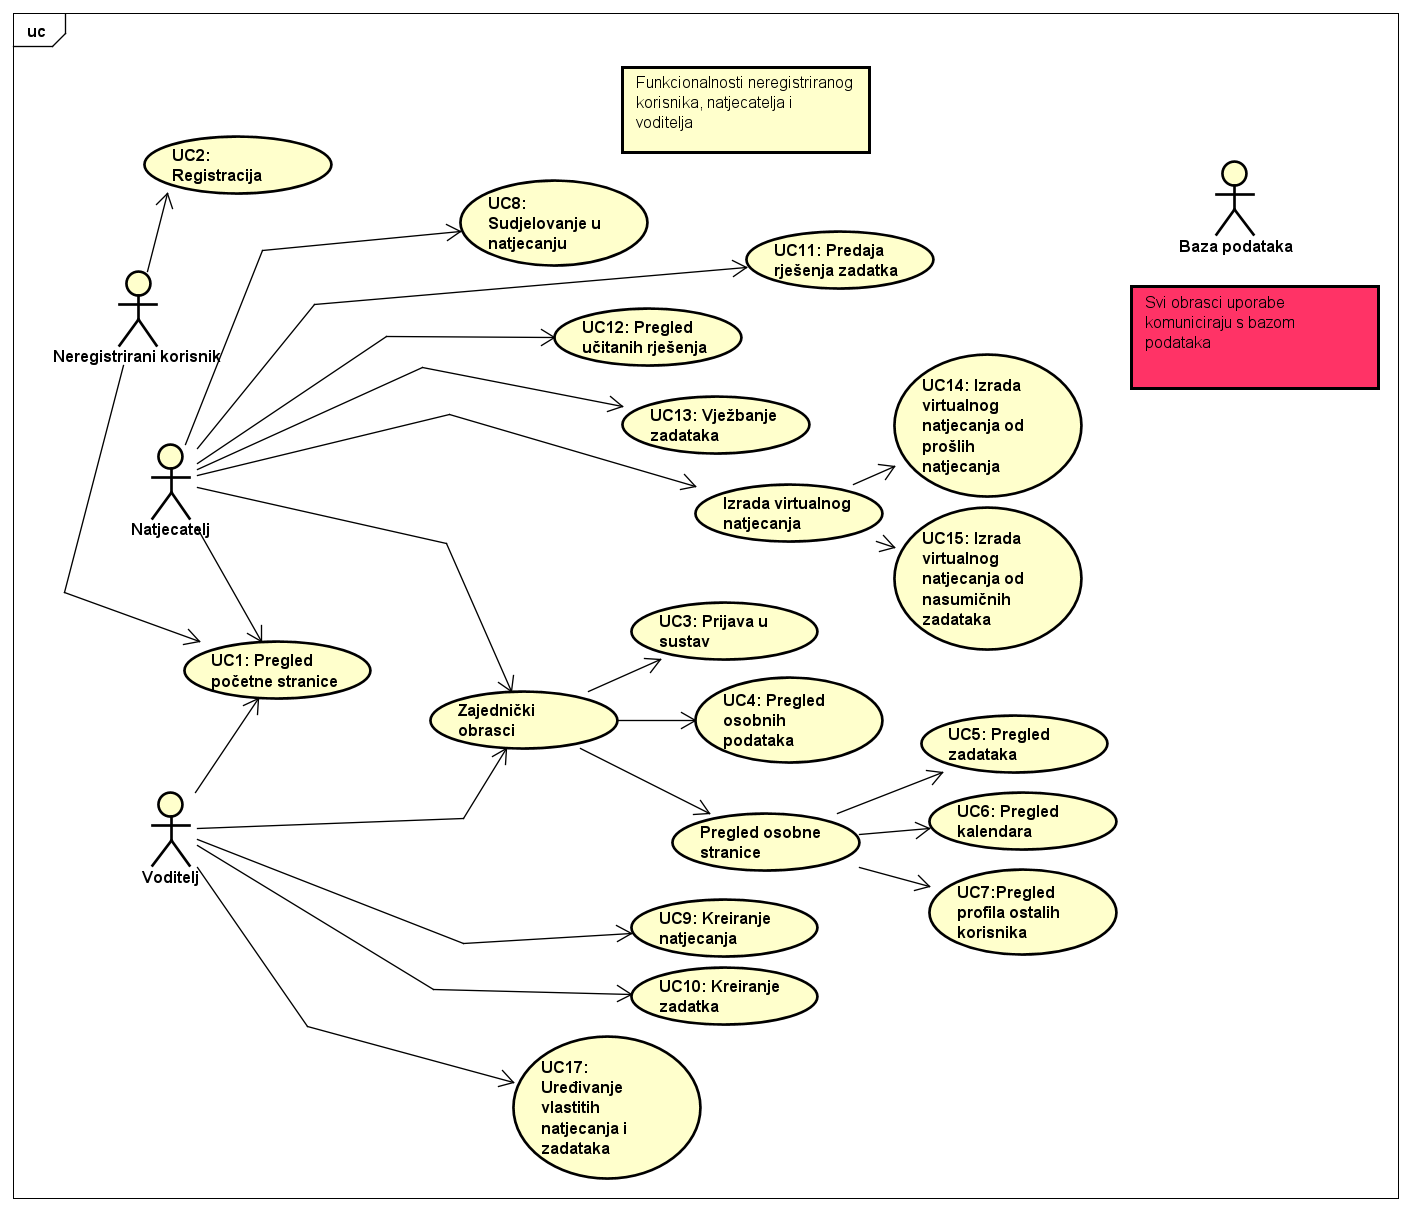
\includegraphics[scale=0.45]{slike/Korisnik_voditelj_natjecatelj.PNG} %veličina slike u odnosu na originalnu datoteku i pozicija slike
						\centering
						\caption{Dijagram obrasca uporabe, fukcionalnost natjecatelja, voditelja i neregistriranog korisnika}
						\label{fig:obrasci1}
					\end{figure}
					
					\eject
					
					\begin{figure}[H]
						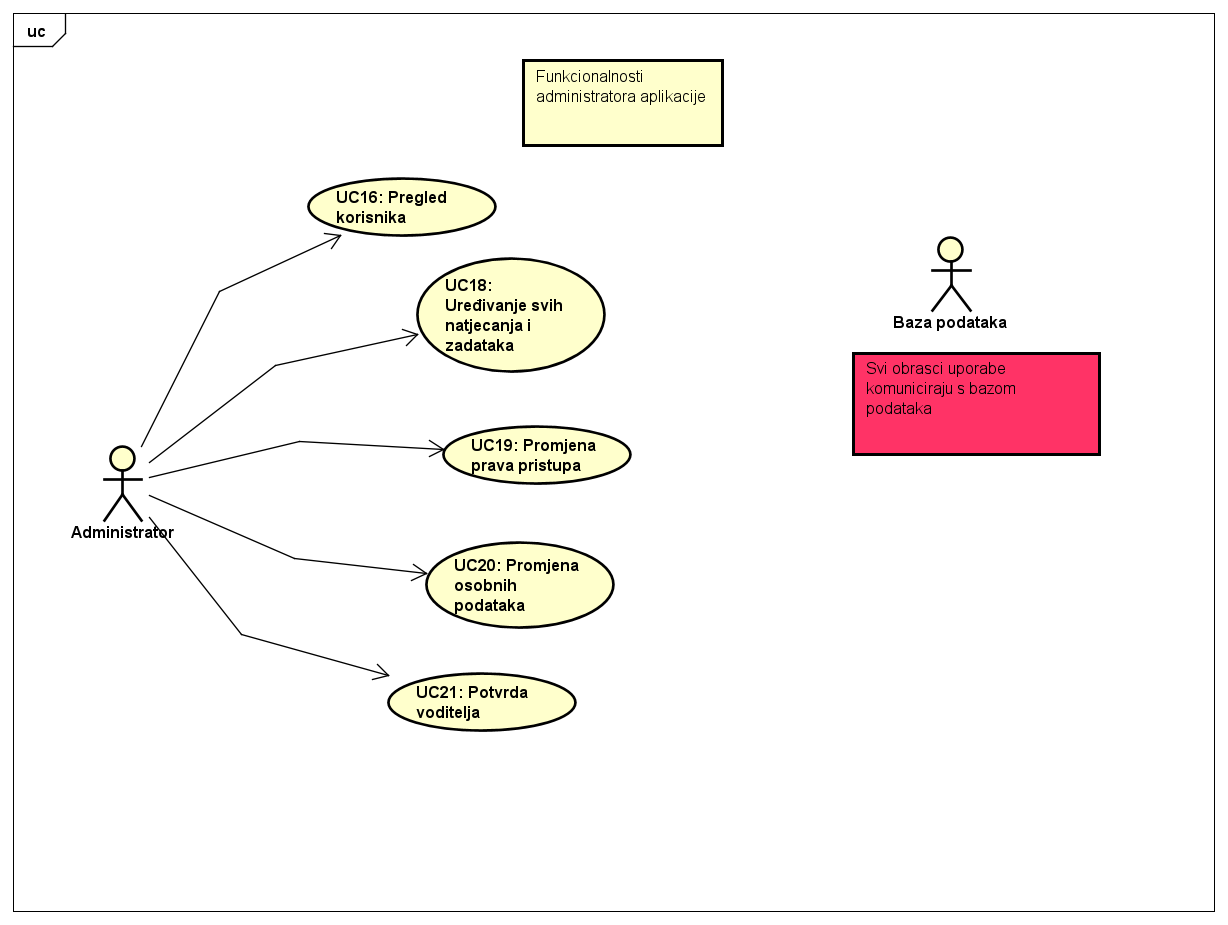
\includegraphics[scale=0.5]{slike/Administrator.PNG} %veličina slike u odnosu na originalnu datoteku i pozicija slike
						\centering
						\caption{Dijagram obrasca uporabe, fukcionalnost administratora}
						\label{fig:obrasci2}
					\end{figure}
				\eject

			\subsection{Sekvencijski dijagrami}

				\vspace{10mm}
				\subsubsection*{UC9 Kreiranje natjecanja}
				
				Voditelj natjecanja započinje proces kreiranja natjecanja slanjem zahtjeva poslužitelju. Poslužitelj provjerava informacije o korisniku u bazi podataka kako bi utvrdila je li korisnik ovlašten za kreiranje natjecanja. Ako je korisnik voditelj natjecanja na web-aplikaciji otvara se forma za izradu natjecanja, voditelj šalje zahtjev za popis dostupnih zadataka, poslužitelj ih dohvaća iz baze podataka i prikazuje ih voditelju. Zatim voditelj odabire željene zadatke i kreira natjecanje. Poslužitelj sprema informacije o natjecanju u bazu podataka i šalje povratnu informaciju voditelju o uspješnom kreiranju natjecanja. Ako korisnik nije voditelj natjecanja poslužitelj šalje odgovor voditelju da samo voditelji natjecanja mogu kreirati natjecanja.
				\vspace{20mm}

				\begin{figure}[htbp]
					\centering
					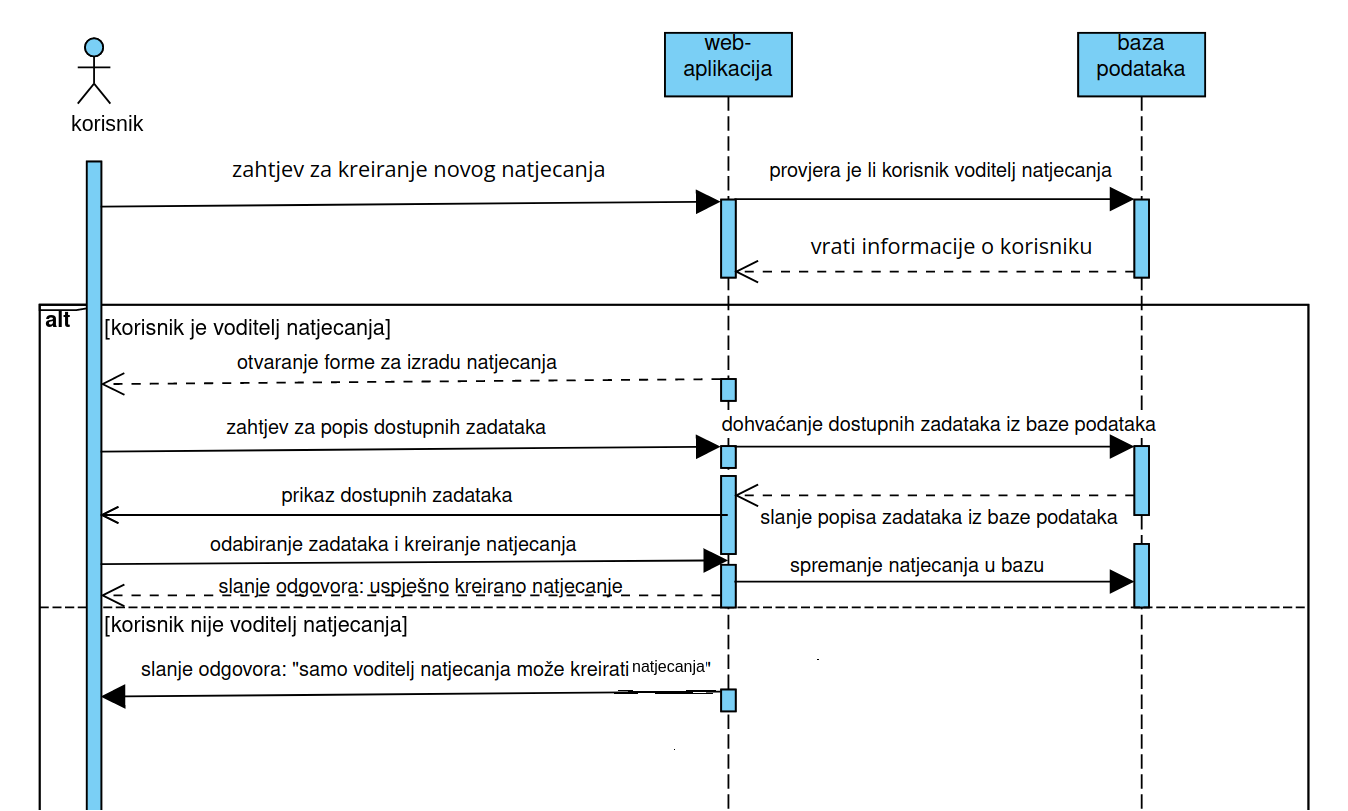
\includegraphics[width=\linewidth]{slike/kreiranje_natjecanja.png}
					\caption{Sekvencijski dijagram kreiranja novog natjecanja}\label{fig:seqdiag_natjecanja}
				\end{figure}
				
				\clearpage 

				\subsubsection*{UC10 Kreiranje zadatka}
				
				Voditelj natjecanja počinje proces kreiranja novog zadatka slanjem zahtjeva poslužitelju koji provjerava je li korisnik voditelj natjecanja. Ako je korisnik voditelj natjecanja poslužitelj omogućuje pristup formi za unos zadatka. Voditelj unosi detalje zadatka i testne primjere te šalje podatke. Poslužitelj prosljeđuje spremanje zadatka u bazu podataka te šalje potvrdu voditelju o uspješnom kreiranju zadatka. Ako korisnik nije voditelj natjecanja poslužitelj šalje poruku korisniku da samo voditelj natjecanja može kreirati zadatke.
				\vspace{20mm}

				\begin{figure}[htbp]
					\centering
					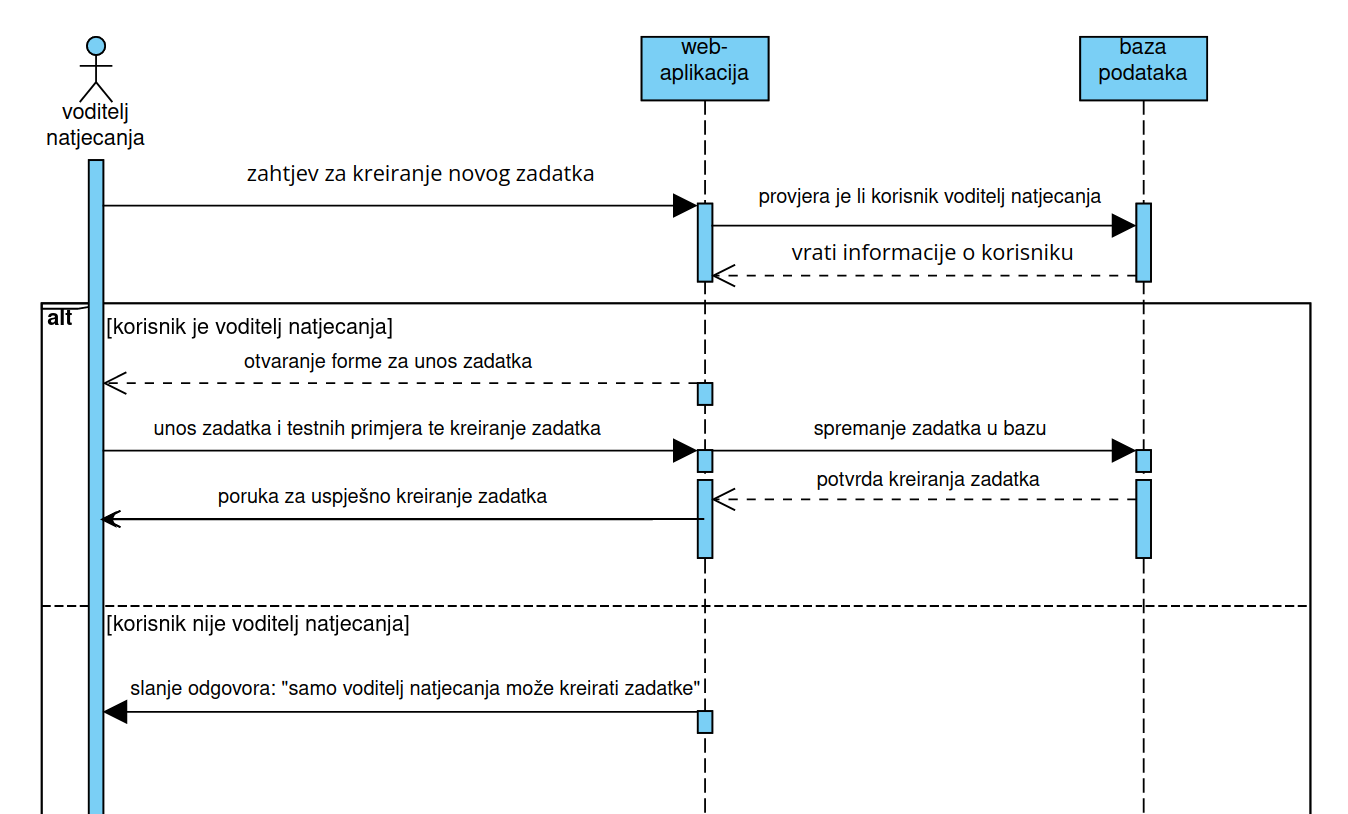
\includegraphics[width=\linewidth]{slike/kreiranje_zadatka.png}
					\caption{Sekvencijski dijagram kreiranja novog zadatka}\label{fig:seqdiag_zadatka}
				\end{figure}
				
				
				\clearpage 
				
				\subsubsection*{UC11 Predaja rješenja}
				
				Natjecatelj započinje proces predaje rješenja zadatka slanjem zahtjeva poslužitelju koji proslijedi zahtjev evaluatoru za pokretanje programa nad testnim primjerima. Evaluator proslijedi zahtjev third party compileru. Compiler pokreće program nad testnim primjerima i šalje rezultate evaluatoru. Evaluator izračunava broj dobivenih bodova i šalje ih Poslužitelju koji ažurira natjecatelja s brojem dobivenih bodova te šalje rezultate i broj bodova bazi podataka za spremanje.
				\vspace{20mm}

				\begin{figure}[htbp]
					\centering
					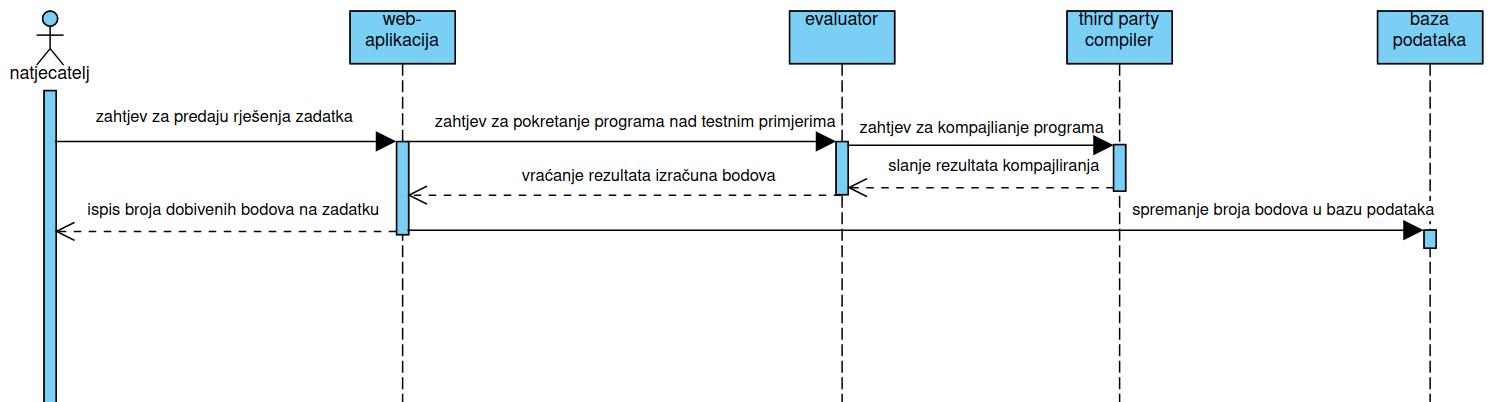
\includegraphics[width=\linewidth]{slike/predaja_rjesenja_zadatka.png}
					\caption{Sekvencijski dijagram predaje rješenja zadatka}\label{fig:seqdiag_rjesenja}
				\end{figure}


			\eject 
	
		\section{Ostali zahtjevi}
		
			\begin{packed_item}
				\item Cijeli sustav namijenjen je upotrebi na engleskom jeziku
				\item Sustav mora biti u mogućnosti podržati veći broj korisnika zbog svoje namjene
				\item Upotreba gotove aplikacije zamišljena je preko web preglednika
				\item Aplikacija mora implementirati autentikaciju i autorizaciju svakog korisnika
				\item Osjetljivi podaci od korisnika se moraju pretvarati u hash prije spremanja u bazu
				\item Greška u jednom dijelu sustava ne smije onemogućiti korištenje drugih usluga
				\item Odgovori sustava prema korisniku moraju biti brzi i ne dulji od nekoliko sekundi
			\end{packed_item}
			 
			 
			 
	